\section{Architecture}

L'architecture de notre logiciel est composée de 4 couches:
\begin{enumerate}
	\item La bibliothèque PresTaf qui permet de manipuler des automates et d'éffectuer des opérations dessus. Nous avons créé une interface en java qui permet d'accéder plus simplement aux fonctions de la bibliothèques.
	\item La première couche Lua est composée des différentes bibliothèques de logique utilisant la bibliothèque Prestaf. Nous avons développé la bibliothèque Presburger.
	\item La deuxième couche Lua contient les différents fichiers des utilisateurs des bibliothèques de logique.
	\item Le Java. C'est le launcher qui permet de démarrer l'application avec une unique commande tout en permettant d'utiliser du java et du Lua.
\end{enumerate}

Ainsi, la première et quatrième couches de l'application font parties de la bibliothèque Prestaf. Il y a deux sortes d'utilisateurs. En effet, une partie des utilisateurs utiliseront directement notre bibliothèque pour développer leur propre bibliothèque de logique, tandis que l'autre partie des utilisateurs utiliseront les bibliothèques de logique. Un utilisateur peut également être utilisateur de sa propre bibliothèque. Le premier groupe d'utilisateur travaillera essentiellement sur la 2\textsuperscript{ème} couche de l'application, tandis que le second groupe travaillera sur la 3\textsuperscript{ème} couche.\\\par

Lua et Java n'étant normalement pas compatible, pour pouvoir interfacer Lua et Java il nous a fallu utiliser une librairie : LuaJava. Cette bibliothèque permet au Java d'executer du Lua et d'altérer sa pile, en ajoutant et modifiant des variables.\\

\begin{figure}[h]
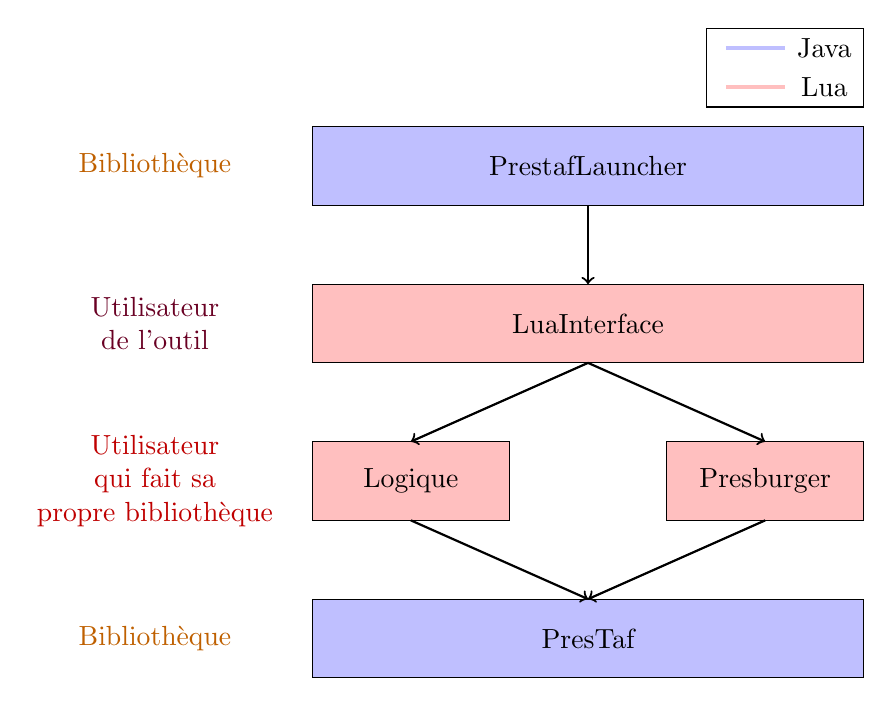
\begin{tikzpicture}

\draw (5, 0.25) rectangle (7, 1.25);
\draw[color=blue!25, ultra thick] (5.25, 1) -- (6, 1);
\draw (6.5, 1) node{Java};
\draw[color=red!25, ultra thick] (5.25, 0.5) -- (6, 0.5);
\draw (6.5, 0.5) node{Lua};

\draw[fill=blue!25] (0,0) rectangle (7,-1);
\draw (3.5, -0.5) node{PrestafLauncher};

\draw[->,thick] (3.5, -1) -- (3.5, -2);

\draw[fill=red!25] (0, -2) rectangle (7, -3);
\draw (3.5, -2.5) node{LuaInterface};

\draw[fill=red!25] (0, -4) rectangle (2.5, -5);
\draw[fill=red!25] (4.5, -4) rectangle (7, -5);
\draw (1.25, -4.5) node{Logique};
\draw (5.75, -4.5) node{Presburger};

\draw[->,thick] (3.5, -3) -- (1.25, -4);
\draw[->,thick] (3.5, -3) -- (5.75, -4);

\draw[fill=blue!25] (0, -6) rectangle (7,-7);
\draw (3.5, -6.5) node{PresTaf};

\draw[->,thick] (1.25, -5) -- (3.5, -6);
\draw[->,thick] (5.75, -5) -- (3.5, -6);

\draw[color=orange!75!black] (-2, -0.5) node[align=center]{Bibliothèque};
\draw[color=purple!55!black] (-2, -2.5) node[align=center]{Utilisateur\\de l'outil};
\draw[color=red!75!black] (-2, -4.5) node[align=center]{Utilisateur\\qui fait sa\\propre bibliothèque};
\draw[color=orange!75!black] (-2, -6.5) node[align=center]{Bibliothèque};

\end{tikzpicture}
\caption{Architecture type de PresTaf et son utilisation}
\end{figure}
